% Chapter 5 from the standard thesis template
%   with a full page figure and a sideways table.
\chapter{SUMMARY AND DISCUSSION}

%This is the opening paragraph to my thesis which
%explains in general terms the concepts and hypothesis
%which will be used in my thesis.
%
%With more general information given here than really
%necessary.
%
%\section{Introduction}
%
%Here initial concepts and conditions are explained and
%several hypothesis are mentioned in brief.
%
%Or graphically as seen in Figure~\ref{mgraph2}
%it is certain that my hypothesis is true.
%
%\begin{figure}[p!] \centering
%
%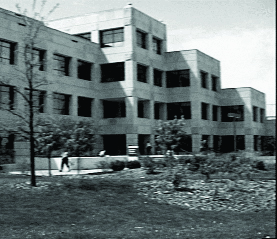
\includegraphics{Images/dc5}
%
%\isucaption{Durham Centre---  Another View}
%\label{mgraph2}
%\end{figure}
%
%\subsection{Hypothesis}
%
%Here one particular hypothesis is explained in depth
%and is examined in the light of current literature.
%
%As can be seen in Table~\ref{nothingelse} it is
%truly obvious what I am saying is true.
%
%\begin{sidewaystable} \centering
%\isucaption{This table shows almost nothing but is a
%sideways table and takes up a whole page by itself}
%\label{nothingelse}
%% Use: \begin{tabular{|lcc|} to put table in a box
%\begin{tabular}{lcc} \hline
%\textbf{Element} & \textbf{Control} & \textbf{Experimental} \\ \hline
%Moon Rings & 1.23 & 3.38 \\
%Moon Tides & 2.26 & 3.12 \\
%Moon Walk & 3.33 & 9.29 \\ \hline
%\end{tabular}
%\end{sidewaystable}
%
%\subsubsection{Parts of the hypothesis}
%
%Here one particular part of the hypothesis that is 
%currently being explained is examined and particular
%elements of that part are given careful scrutiny.
%
%% Below \subsubsection
%% Sectional commands: \paragraph and \subparagraph may also be used
%
%\subsection{Second Hypothesis}
%
%Here one particular hypothesis is explained in depth
%and is examined in the light of current literature.
%
%\subsubsection{Parts of the second hypothesis}
%
%Here one particular part of the hypothesis that is 
%currently being explained is examined and particular
%elements of that part are given careful scrutiny.
%
%\section{Criteria Review}
%
%Here certain criteria are explained thus eventually
%leading to a foregone conclusion.

